\documentclass{standalone}
\usepackage{tikz}
\begin{document}
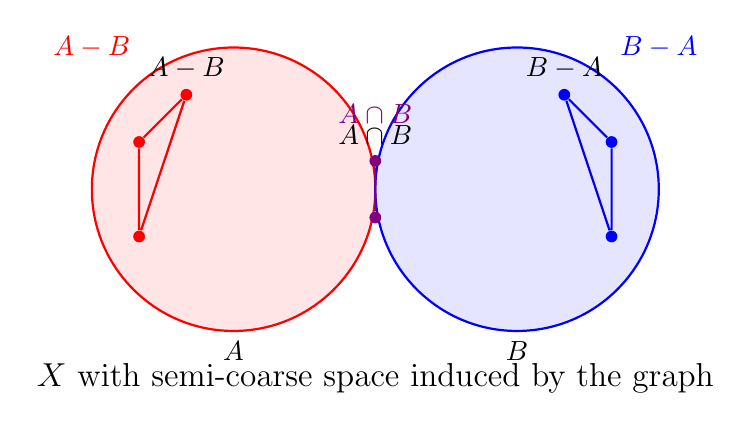
\begin{tikzpicture}[scale=1.2]
  % Draw sets A and B as overlapping circles
  \draw[fill=red!10, draw=red, thick] (0,0) circle (1.5cm) node[below=1.8cm] {$A$};
  \draw[fill=blue!10, draw=blue, thick] (3,0) circle (1.5cm) node[below=1.8cm] {$B$};
  
  % Points in A-B (red)
  \node[red, circle, fill, inner sep=1.5pt, label=above:{$A-B$}] (A1) at (-0.5, 1) {};
  \node[red, circle, fill, inner sep=1.5pt] (A2) at (-1, 0.5) {};
  \node[red, circle, fill, inner sep=1.5pt] (A3) at (-1, -0.5) {};
  
  % Points in B-A (blue)
  \node[blue, circle, fill, inner sep=1.5pt, label=above:{$B-A$}] (B1) at (3.5, 1) {};
  \node[blue, circle, fill, inner sep=1.5pt] (B2) at (4, 0.5) {};
  \node[blue, circle, fill, inner sep=1.5pt] (B3) at (4, -0.5) {};
  
  % Points in A∩B (violet)
  \node[violet, circle, fill, inner sep=1.5pt, label=above:{$A \cap B$}] (C1) at (1.5, 0.3) {};
  \node[violet, circle, fill, inner sep=1.5pt] (C2) at (1.5, -0.3) {};
  
  % Graph edges: Connect points within each set
  \draw[red, thick] (A1) -- (A2) -- (A3) -- (A1); % Triangle in A-B
  \draw[blue, thick] (B1) -- (B2) -- (B3) -- (B1); % Triangle in B-A
  \draw[violet, thick] (C1) -- (C2); % Line in A∩B
  
  % Labels for regions
  \node at (-1.5, 1.5) {\textcolor{red}{$A-B$}};
  \node at (4.5, 1.5) {\textcolor{blue}{$B-A$}};
  \node at (1.5, 0.8) {\textcolor{violet}{$A \cap B$}};
  
  % Title
  \node at (1.5, -2) {\large$X$ with semi-coarse space induced by the graph};
\end{tikzpicture}
\end{document}